\documentclass[12pt,a4paper]{article}

% Paquetes básicos
\usepackage[utf8]{inputenc}
\usepackage[spanish]{babel}
\usepackage{graphicx}
\usepackage{amsmath}
\usepackage{amssymb}
\usepackage{hyperref}
\usepackage{geometry}
\usepackage{listings}
\usepackage{xcolor}
\usepackage{float}

% Configurar márgenes
\geometry{
    top=2.5cm,
    bottom=2.5cm,
    left=3cm,
    right=3cm
}

% Configuración de listings para código Python
\lstset{
    language=Python,
    basicstyle=\ttfamily\small,
    keywordstyle=\color{blue},
    commentstyle=\color{green!60!black},
    stringstyle=\color{red},
    breaklines=true,
    frame=single,
    numbers=left,
    numberstyle=\tiny\color{gray}
}

% Información del documento
\title{Práctica 1: Aprendizaje por Refuerzo en Robobo\\
\large Robótica Inteligente Aplicada}
\author{Marcelo Ferreiro Sánchez\\ Pepe Romero Conde}
\date{\today}

\begin{document}

\maketitle

\tableofcontents

\newpage

\section{Introducción}

Esta práctica consiste en la implementación de un entorno de aprendizaje por
refuerzo utilizando el framework Gymnasium para controlar un robot Robobo
simulado. El objetivo es que el robot aprenda a seguir un objeto móvil (blob)
optimizando su comportamiento mediante recompensas.

\section{Descripción del entorno}

\subsection{Espacio de observación}

El entorno proporciona al agente información sobre el estado actual mediante un
espacio de observación, implementado como un diccionario. Contiene cuatro
partes principales que describen el estado del sistema. La primera
parte, denominada \textbf{blob\_xy}, proporciona las coordenadas $(x, y)$
del blob detectado por la cámara, con valores en el rango $[-1, 102]$. El valor
especial $-1$ indica que el blob no está visible en el campo visual del robot.
La segunda parte corresponde a los sensores \textbf{IR}, que proporcionan
lecturas de los sensores infrarrojos frontal y trasero con valores en el rango
$[0, 1000]$, clave para saber si el robot está cerca de una pared. La tercera parte es el \textbf{tamano\_blob}, que representa el
tamaño aparente del blob medido en píxeles, con valores en el rango $[0, 1000]$.
Un tamaño mayor indica que el robot está más cerca del objeto objetivo.
Finalmente, \textbf{velocidad} contiene las velocidades actuales
de las ruedas izquierda y derecha, con valores en el rango $[-2, 2]$.

\subsection{Espacio de acciones}

El espacio de acciones es continuo y bidimensional, definido como un
\texttt{Box} con valores en el intervalo $[-2, 2]^2$. El primer componente de
cada acción representa el avance recto, donde valores positivos provocan avance
hacia adelante y valores negativos producen retroceso. El segundo
controla el giro, donde valores positivos generan rotación a la derecha y
valores negativos producen rotación a la izquierda. Esta representación pone de manifiesto nuestra creencia a que las acciones más fundamentales son ``avanzar'' y ``girar''. Ambas requieren una sincronización entre ambas ruedas, por eso, al representar la acción de esta forma conseguimos que Robobo no tenga que aprender esa sincronización. 

Las velocidades finales de las ruedas se calculan:
\begin{align}
v_{\text{izq}} &= v_{\text{anterior\_izq}} + (\text{avance} + \text{giro}) \\
v_{\text{der}} &= v_{\text{anterior\_der}} + (\text{avance} - \text{giro})
\end{align}

Se recortan al rango admisible $[-2, 2]$ con \texttt{np.clip}.

\subsection{Función de recompensa}

La función de recompensa está diseñada para incentivar múltiples comportamientos
deseables mediante la combinación de cuatro términos. Se define:

\begin{equation}
R = \alpha_1 \cdot e^{-(descentre)^2} + \alpha_2 \cdot e^{-\left(\frac{d}{\sigma}\right)^2} - \alpha_3 \cdot \theta(IR_{\text{atras}} - 58) + \alpha_4 \cdot \text{tamano\_blob}
\end{equation}

Donde
\begin{itemize}
	\item $descentre := x_{blob} - 50$, mide cuanto se aleja el blob del centro de la pantalla. Si justo esta en el centro, $x_{blob}$ = 50 y por tanto $descentre$ = 0, con lo que la recompensa es máxima.
	\item $\sigma$ es un hiperparámetro que controla la agresividad del decaimiento, su diferencia con $\alpha_3$ esque el último dice cuanto peso tiene ese término en la recompensa y el primero el valor del término en sí. Experimentalmente encontramos bueno el valor de 35.
	\item $\theta(x)$ es la función max(0, $x$)
	\item $\alpha \in \mathbb{R}^4$ es el hiperparámetro de ponderación, experimentalmente encontramos como aceptable el valor [2.5, 0.6, 0.0001, 0.1].
\end{itemize}

El primer término, $\alpha_1 \cdot e^{-(descentre)^2}$, proporciona una recompensa gaussiana por mantener el blob centrado horizontalmente en la imagen. El valor óptimo se alcanza cuando $x = 50$, es decir, cuando el objeto se encuentra en el centro del campo visual. El segundo término, $\alpha_2 \cdot e^{-(d/\sigma)^2}$, recompensa la proximidad al blob mediante una función gaussiana de la distancia euclidiana $d$ al objeto, donde el parámetro $\sigma$ controla la escala espacial de la recompensa. El tercer término, $-\alpha_3 \cdot \theta (IR_{\text{atras}} - 58)$, introduce una penalización cuando el sensor infrarrojo trasero detecta obstáculos, evitando así colisiones durante maniobras de retroceso. Como de forma basal el sensor da 57 (y valores más altos cuando tiene el blob o una pared cerca) le restamos 58 y aplicamos la función $\theta (x)$, son estos valores resultantes los que penalizan. Finalmente, el cuarto término, $0.1 \cdot \text{tamano\_blob}$, supone una recompensa proporcional al tamaño aparente del blob, incentivando activamente la aproximación al objeto.


\subsection{Dinámica del episodio}

Cada episodio tiene una duración fija \footnote{Ajustable en \texttt{config.yaml}.} de 60 pasos temporales. Al finalizar cada
paso se ejecuta la acción seleccionada por el agente y se actualiza el estado
del robot en el simulador mediante el envío de comandos de velocidad a las
ruedas. Posteriormente, el blob se mueve de forma aleatoria siguiendo un patrón
de random walk en diagonal. Tras estos
movimientos, se calculan las nuevas observaciones leyendo los sensores del robot
y se evalúa la función de recompensa para proporcionar feedback al agente.
Finalmente, las posiciones del robot y del objeto se almacenan en estructuras de
datos para su posterior análisis y visualización.

\subsection{Historial y seguimiento}

El entorno mantiene tres estructuras de datos que almacenan información completa
de todos los episodios ejecutados. El primero, denominado
\texttt{historial\_recompensas}, es una lista de listas que contiene las
recompensas obtenidas en cada paso de cada episodio. El segundo,
\texttt{historial\_xy\_objeto}, registra las posiciones del blob a lo largo del
tiempo. El tercero, \texttt{historial\_xy\_robot}, almacena las posiciones del
robot durante toda la ejecución. Estos datos históricos permiten realizar
análisis detallados del proceso de aprendizaje del agente y visualizar las
trayectorias seguidas tanto por el robot como por el objeto objetivo.

\section{Implementación técnica}

\subsection{Interfaz con el simulador}

El entorno se comunica con Robobo a través del módulo \texttt{RoboboAPI}, que
proporciona una interfaz completa para la interacción con el robot. Esta
interfaz incluye funciones para conectar con el robot físico mediante la clase
\texttt{Robobo} y con el simulador mediante la clase \texttt{RoboboSim}. Además,
permite leer diversos sensores como la posición del blob, los sensores
infrarrojos y el tamaño del blob en la imagen. También proporciona control sobre
los actuadores, específicamente las velocidades de las ruedas y la posición del
tilt de la cámara. La API incluye métodos para obtener posiciones
globales tanto del robot como del objeto en el mundo simulado, así como para
calcular distancias euclidianas entre ambos elementos.

Estas decisiones de programación fueron tomadas siguiendo la filosofía de Separación de Intereses (\emph{Separation of concerns}, en inglés) de Edsger W. Dijkstra.

\subsection{Método \texttt{reset}}

Al inicio de cada episodio, el método \texttt{reset} se encarga de preparar el
entorno para una nueva secuencia de interacciones. Primero guarda el historial
del episodio anterior en las listas globales de almacenamiento. Después,
reinicia el simulador a su estado inicial. La
cámara del robot se posiciona a 105° para ver mejor el
blob (aunque encontramos que si está muy cerca sigue sin poderlo ver correctamente, argumentablemente un defecto de Robobo). Seguidamente se leen las observaciones iniciales desde los sensores del
robot. Las posiciones iniciales tanto del robot como del objeto se registran en
los historiales correspondientes. Finalmente, el método retorna la observación
inicial al agente para que pueda comenzar el proceso de toma de decisiones.

\subsection{Método \texttt{step}}

En cada paso de tiempo, el método \texttt{step} gestiona la transición del
entorno desde el estado actual al siguiente. Primero recibe la acción
seleccionada por el agente y calcula las nuevas velocidades de las ruedas
aplicando las ecuaciones de control diferencial previamente descritas. Estas
velocidades se envían al robot y el movimiento se ejecuta durante un intervalo
de 1 segundo. Tras completarse el movimiento del robot, el blob se desplaza de
forma aleatoria según el patrón de random walk implementado \footnote{La velocidad a la que se mueve el blob puede ser ajustada en \texttt{config.yaml}}. A continuación se
actualizan todas las observaciones mediante la lectura de los sensores y se
evalúa la función de recompensa utilizando el nuevo estado. Las posiciones
actuales y la recompensa obtenida se almacenan en los historiales
correspondientes. Finalmente, el método determina si el episodio ha alcanzado su
condición de terminación y retorna al agente la observación actualizada, la
recompensa obtenida, los flags de terminación y truncamiento, y un diccionario
con información adicional del paso.

\subsection{¿Cómo ejecutar?}


\begin{lstlisting}[language=bash]
git clone https://github.com/PepeRoConde/RIA
python3 -m venv entornoFerreiroRomero
source entornoFerreiroRomero/bin/activate
pip install -r requirements.txt
python P1/codigo/main.py
\end{lstlisting}

Los hiperparámetros que condicionan la ejecución pueden ser modificados en \texttt{config.yaml}. En caso de que se quiera probar (sin aprendizaje) se debera especificar \texttt{learn: False} en dicho archivo.   

\section{Resultados y análisis}

\subsection{Visualizaciones}

Para analizar el comportamiento del agente se implementaron funciones de
visualización específicas. Estas funciones permiten generar gráficas de las
trayectorias del robot y del objeto en el plano $xy$, facilitando entender el
movimiento. También se incluye la visualización de la evolución de las
recompensas a lo largo de los episodios, permitiendo evaluar el progreso del
aprendizaje. 
\subsection{Comportamiento esperado}

Un agente correctamente entrenado debería exhibir varios comportamientos
característicos. En primer lugar, debería ser capaz de mantener el blob centrado
en su campo visual, ajustando continuamente su orientación. Además, debería
seguir al blob cuando este se mueve por el entorno, demostrando
capacidad de seguimiento. 
Idealmente, debería desarrollar estrategias para evitar colisiones con
obstáculos, especialmente durante maniobras de retroceso, utilizando
los sensores infrarrojos.

\section{Conclusiones}

Si bien el robot no presenta un comportamiento tan bueno como la demo que presentó el profesor en clase, se considera que se puede demostrar que, efectivamente, ha aprendido un comportamiento más o menos inteligente. La función de coste efectivamente ha dirigido las acciones del robot hacia las deseadas, de forma más o menos rápida y, con el suficiente tiempo para experimentar, creemos que sería posible alcanzar un mejor comportamiento a base de prueba y error con los diferentes parámetros.
Se observa cómo el robot rara vez consigue agarrar el objeto completamente pues parte de su función de recompensa consta del tamaño del blob, el cual disminuirá al encontrarse muy cerca del mismo, pues dejará de estar en su campo de visión. Una forma de arreglar este problema podría ser anular tal parte de la recompensa tras cierto tamaño de blob, e incluir como incentivo las activaciones del sensor IR delantero por ejemplo. Igualmente viendo las gráficas apreciamos cómo el robot busca siempre al blob y mantenerse cerca de el mismo.

\begin{figure}[h]
    \centering
    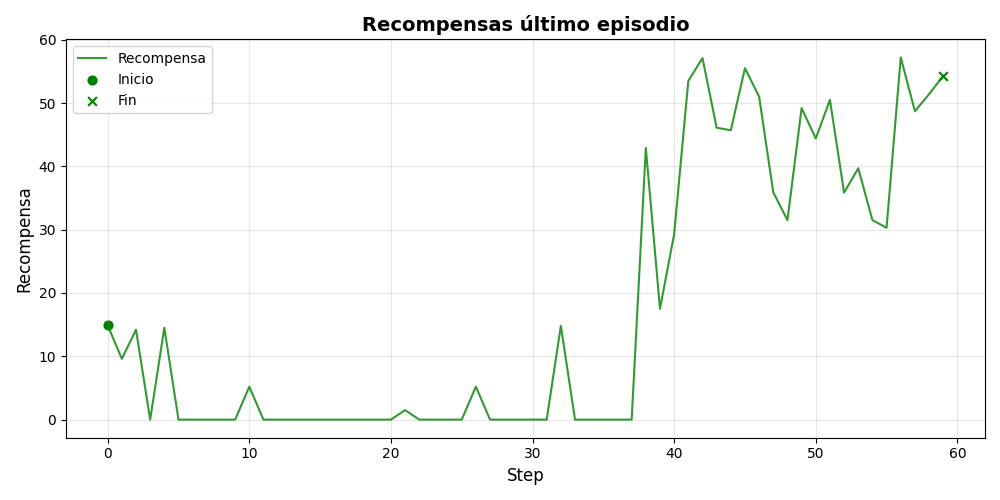
\includegraphics[width=0.8\textwidth]{Figure_1.png}
    \caption{Evolución de las recompensas en el último episodio de entrenamiento}
    \label{fig:etiqueta}
\end{figure}

\begin{figure}[h]
    \centering
    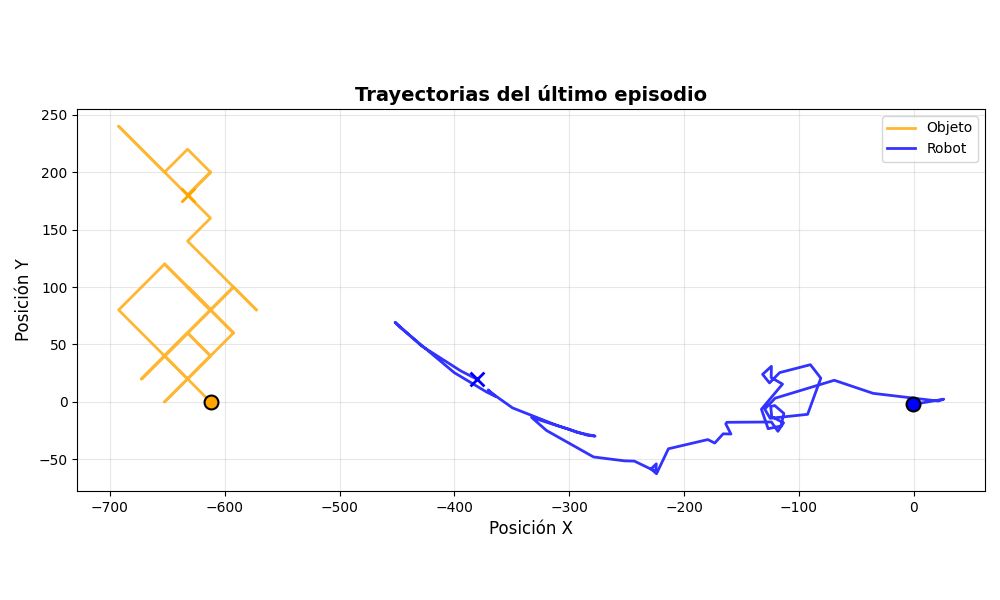
\includegraphics[width=0.8\textwidth]{Figure_12.png}
    \caption{Trayectorias del blob y robot en el último episodio.}
    \label{fig:etiqueta2}
\end{figure}

\subsection{Trabajo futuro}

Ajustar más aún las funcion de coste y el número  de episodios de entrenamiento
apra aproximarse al comportamiento que implementó el profesor. También pensar en
aumentar la velocidad máxima del robot hasta sus propios límites físicos
$[-100,100]$ o hasta que el simulador comience a dar errores.
Explorar, en general el espacio de hiperparámetros y ejecuciones de entrenamiento más largas. Estas cuestiones mejoraran el rendimiento de nuestro agente, pero, por el contrario no contribuirán a un mayor aprendizaje sobre la materia por lo que reconocemos que el tiempo que dedicamos a dichas tareas fue un compromiso entre el necesario para que Robobo mostrase un buen comportamiento y estar horas cambiando hiperparámetros para ver si mejora un poco más. 
\end{document}
